\chapter{Application Specifications}

In this chapter, I have listed the features of the Client app, as well as which features were discarded and justifications for doing so.

\section{Implemented Features}

Using this app, students can borrow (with or without a deposit) and sell items amongst themselves (Figure \ref{fig:lend}). They can search for their desired item from a list (Figure \ref{fig:homepage}) via text based search (Figure \ref{fig:search}) or from a list of categories (Figure \ref{fig:category}) as well as add their own items with textual details and pictures (Figure \ref{fig:add}, \ref{fig:gallery-select}). Users can navigate the app using a slide-in menu to other pages (Figure \ref{fig:menu}), e.g. their profile where they find their avatars, simple ratings, items and comments by others (Figure \ref{fig:profile}). They also receive push notifications about items they want to borrow/sell and find a list of such notifications in app (Figure \ref{fig:notification}, \ref{fig:requests}).

\section{Unimplemented Features}

This project is not about creating a production ready app, but rather to investigate and experience software engineering(SE) practices. If some feature did not add to a high-priority user story or did not add to the SE values, then it was ignored. Some of the important ones are below - 

\begin{itemize}
	\item Users cannot create their own accounts, i.e. there is no registration.  One reason to do so is that, I imagined such a system to use the university authentication to guarantee that only UoS students use the service. Although, there is a REST route available on the server side to do it, so that, on the first login in a production app, a User object will be created on the database.
	
	\item There is no chatting option on the app, even though the placement in the UI is there. The major reasons are - time constraints and less priority. Given the choice between push notification and chat, the user interviews led me to (rightly) prioritise push. I discuss more about it in later chapters.
	
	\item Users cannot upload a profile picture, a default one is set for them. For demo purposes, I edited user objects on the database myself in the figures here. I have demonstrated how such features can be implemented by allowing to upload item picture, so other user stories took priority.
\end{itemize}

\section{Screenshots}
\begin{figure}[!h]
    \centering
    \begin{subfigure}[b]{0.3\textwidth}
        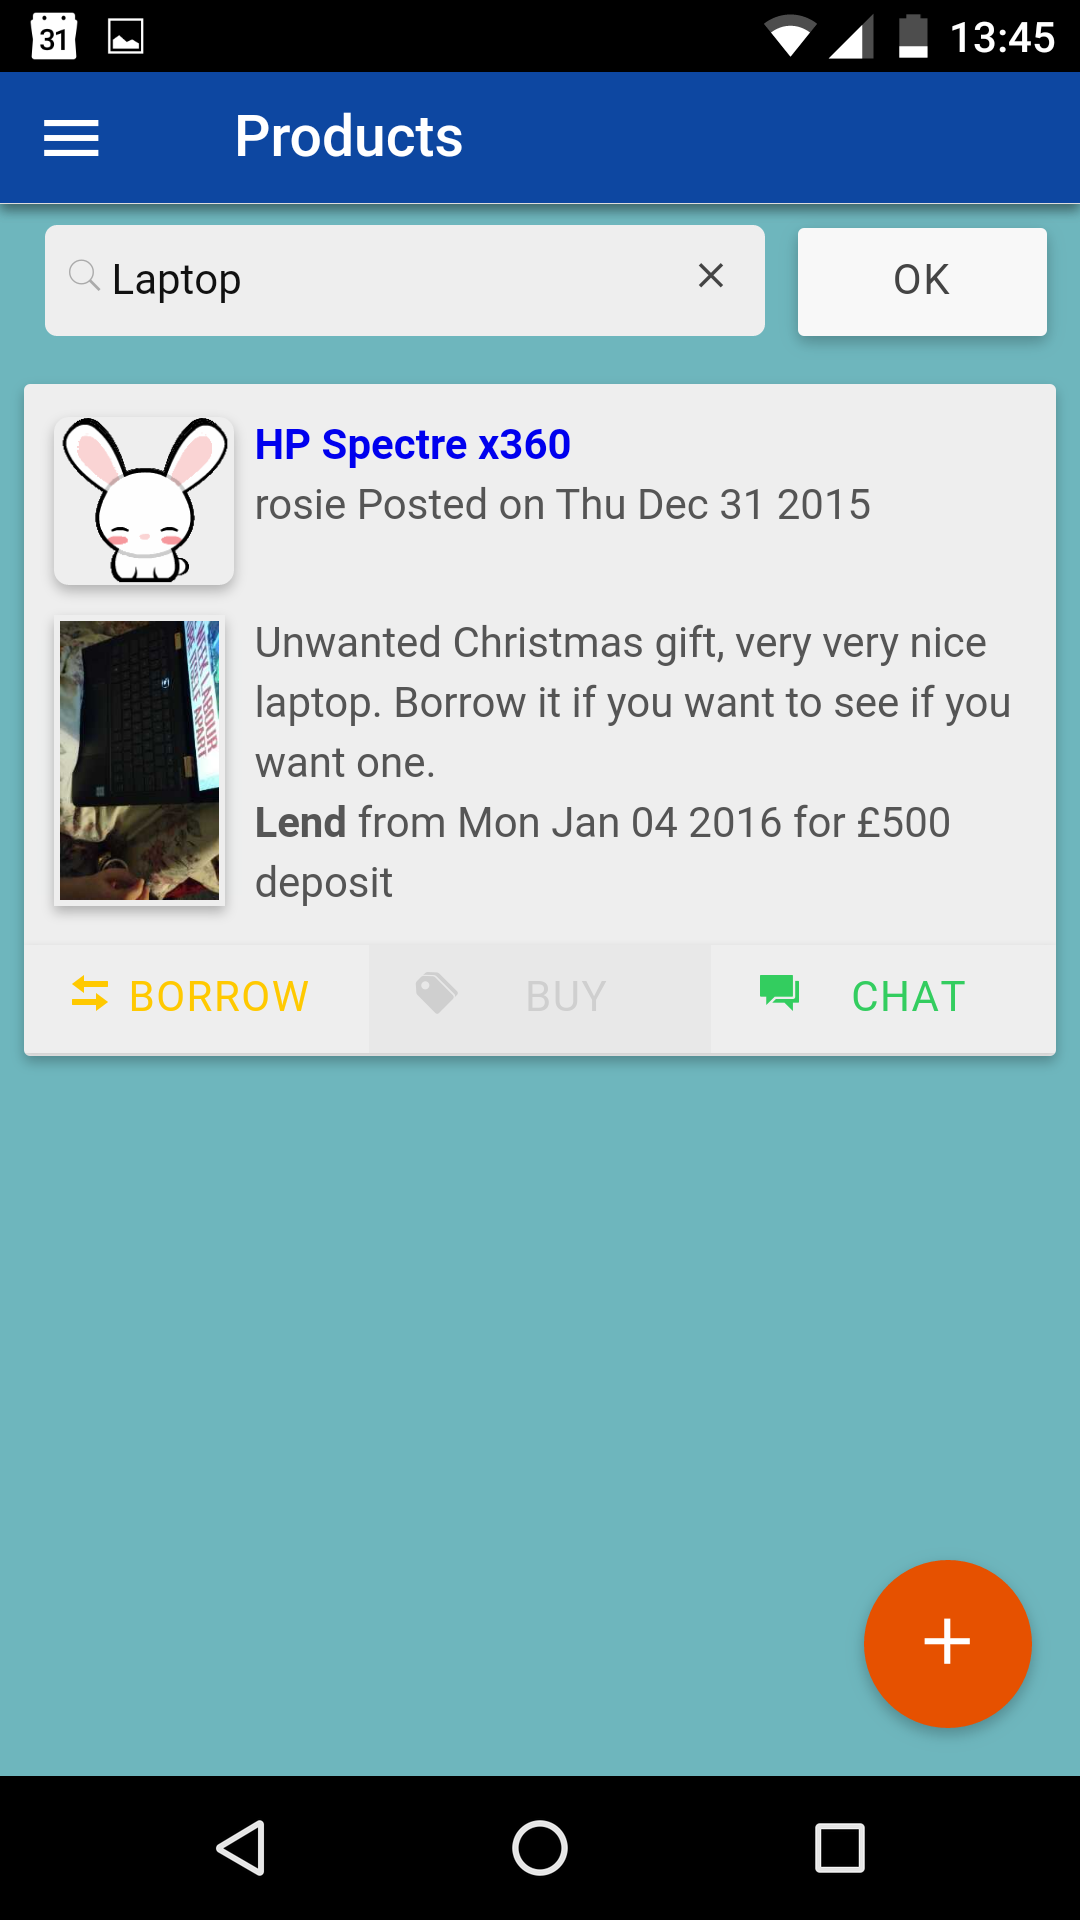
\includegraphics[width=\textwidth]{search}
        \caption{Search}
        \label{fig:search}
    \end{subfigure}
    ~
    \begin{subfigure}[b]{0.3\textwidth}
        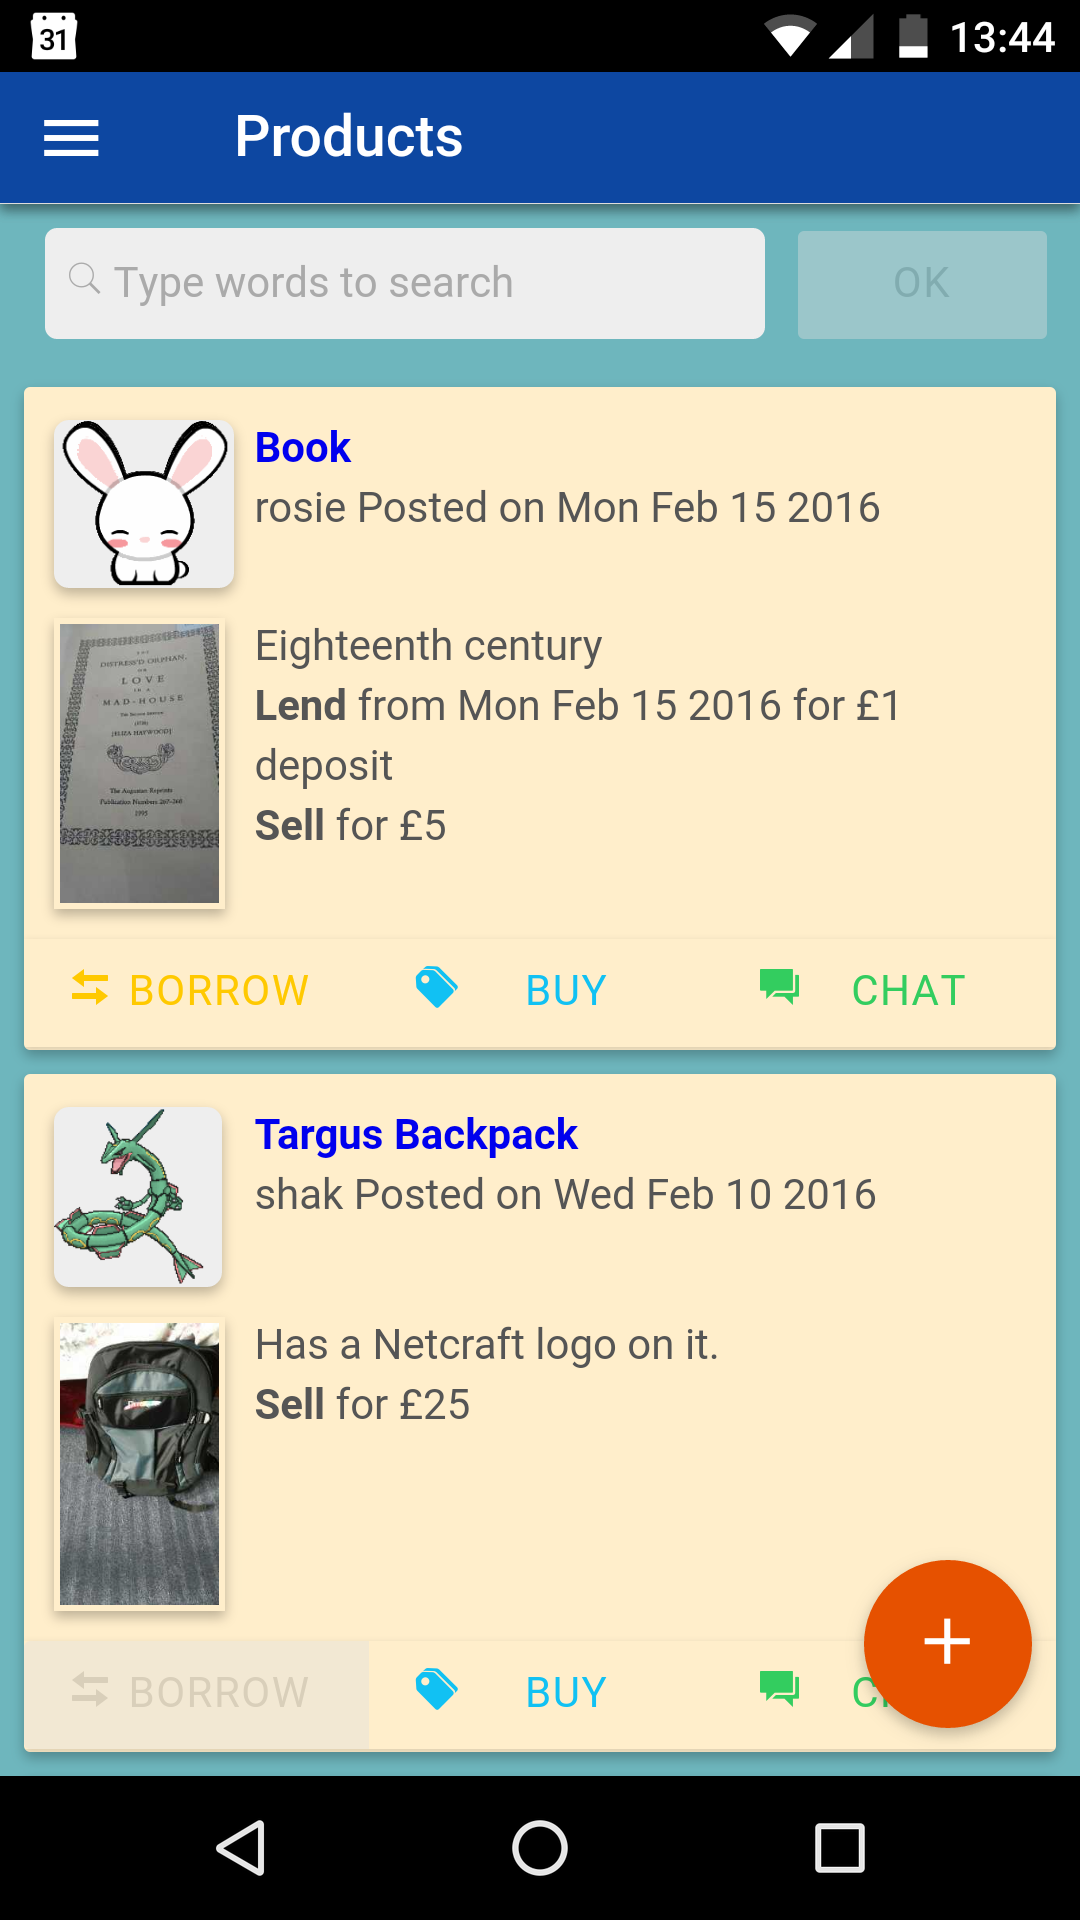
\includegraphics[width=\textwidth]{homepage}
        \caption{Product List}
        \label{fig:homepage}
    \end{subfigure}
    ~
    \begin{subfigure}[b]{0.3\textwidth}
        
\includegraphics[width=\textwidth]{menu}
        \caption{Menu}
        \label{fig:menu}
    \end{subfigure}
    \caption{Screenshots}\label{fig:scr3}
\end{figure}
\begin{figure}[!h]
    \centering
    \begin{subfigure}[b]{0.3\textwidth}
        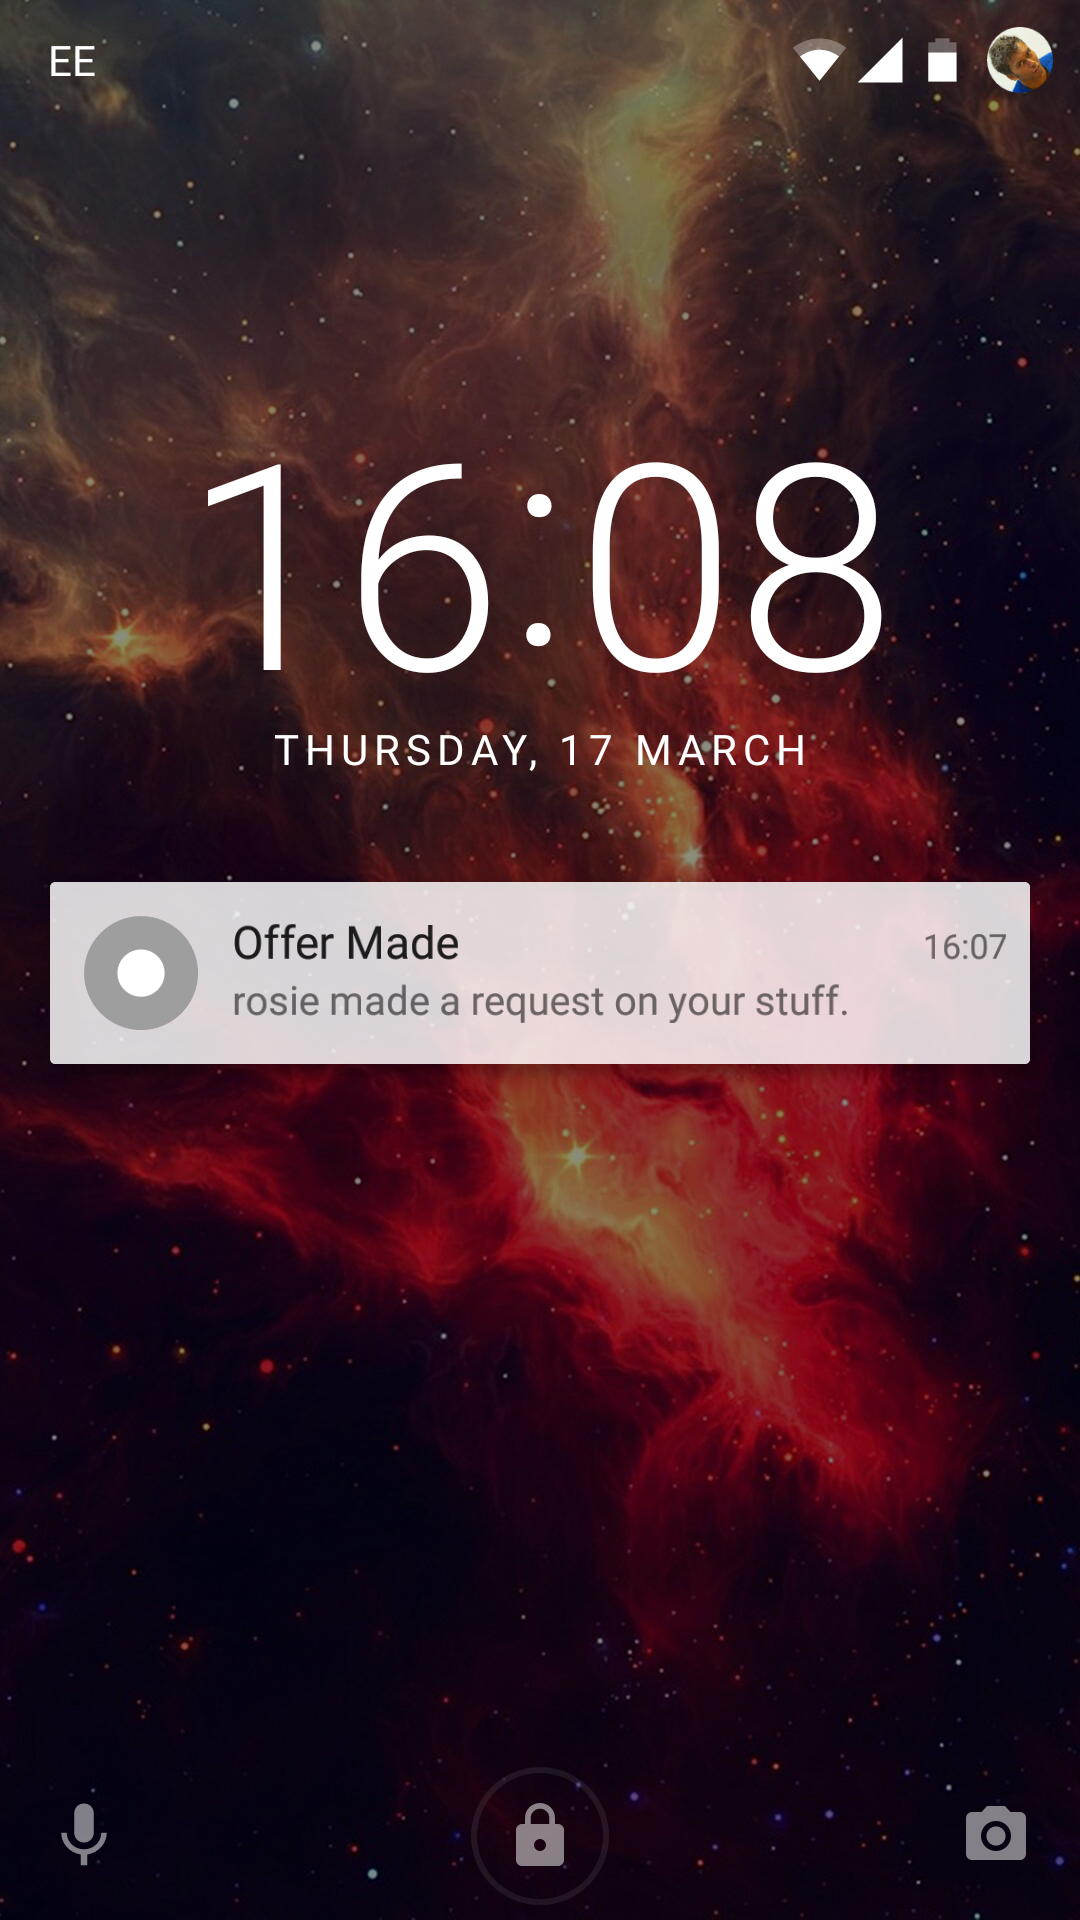
\includegraphics[width=\textwidth]{notification}
        \caption{Notification}
        \label{fig:notification}
    \end{subfigure}
    ~
    \begin{subfigure}[b]{0.3\textwidth}
        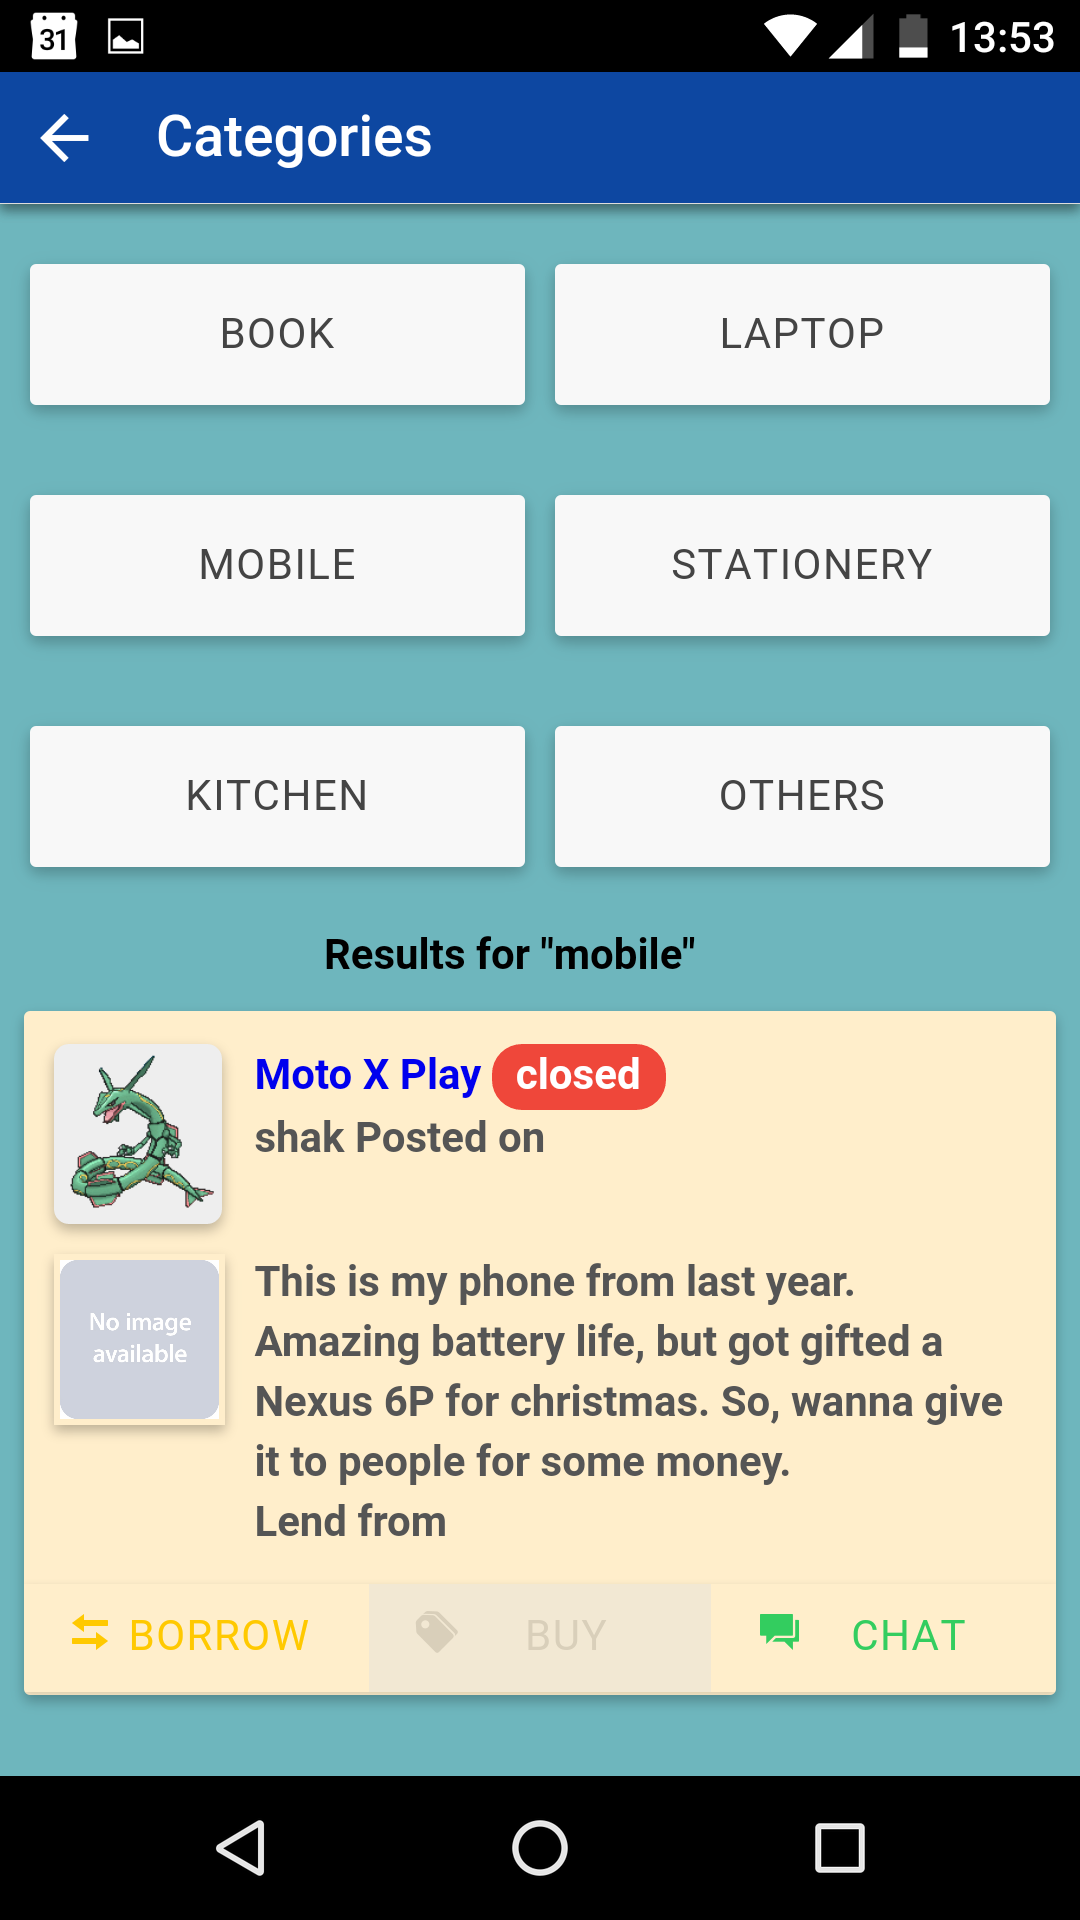
\includegraphics[width=\textwidth]{category}
        \caption{Category List}
        \label{fig:category}
    \end{subfigure}
    ~
   \begin{subfigure}[b]{0.3\textwidth}
        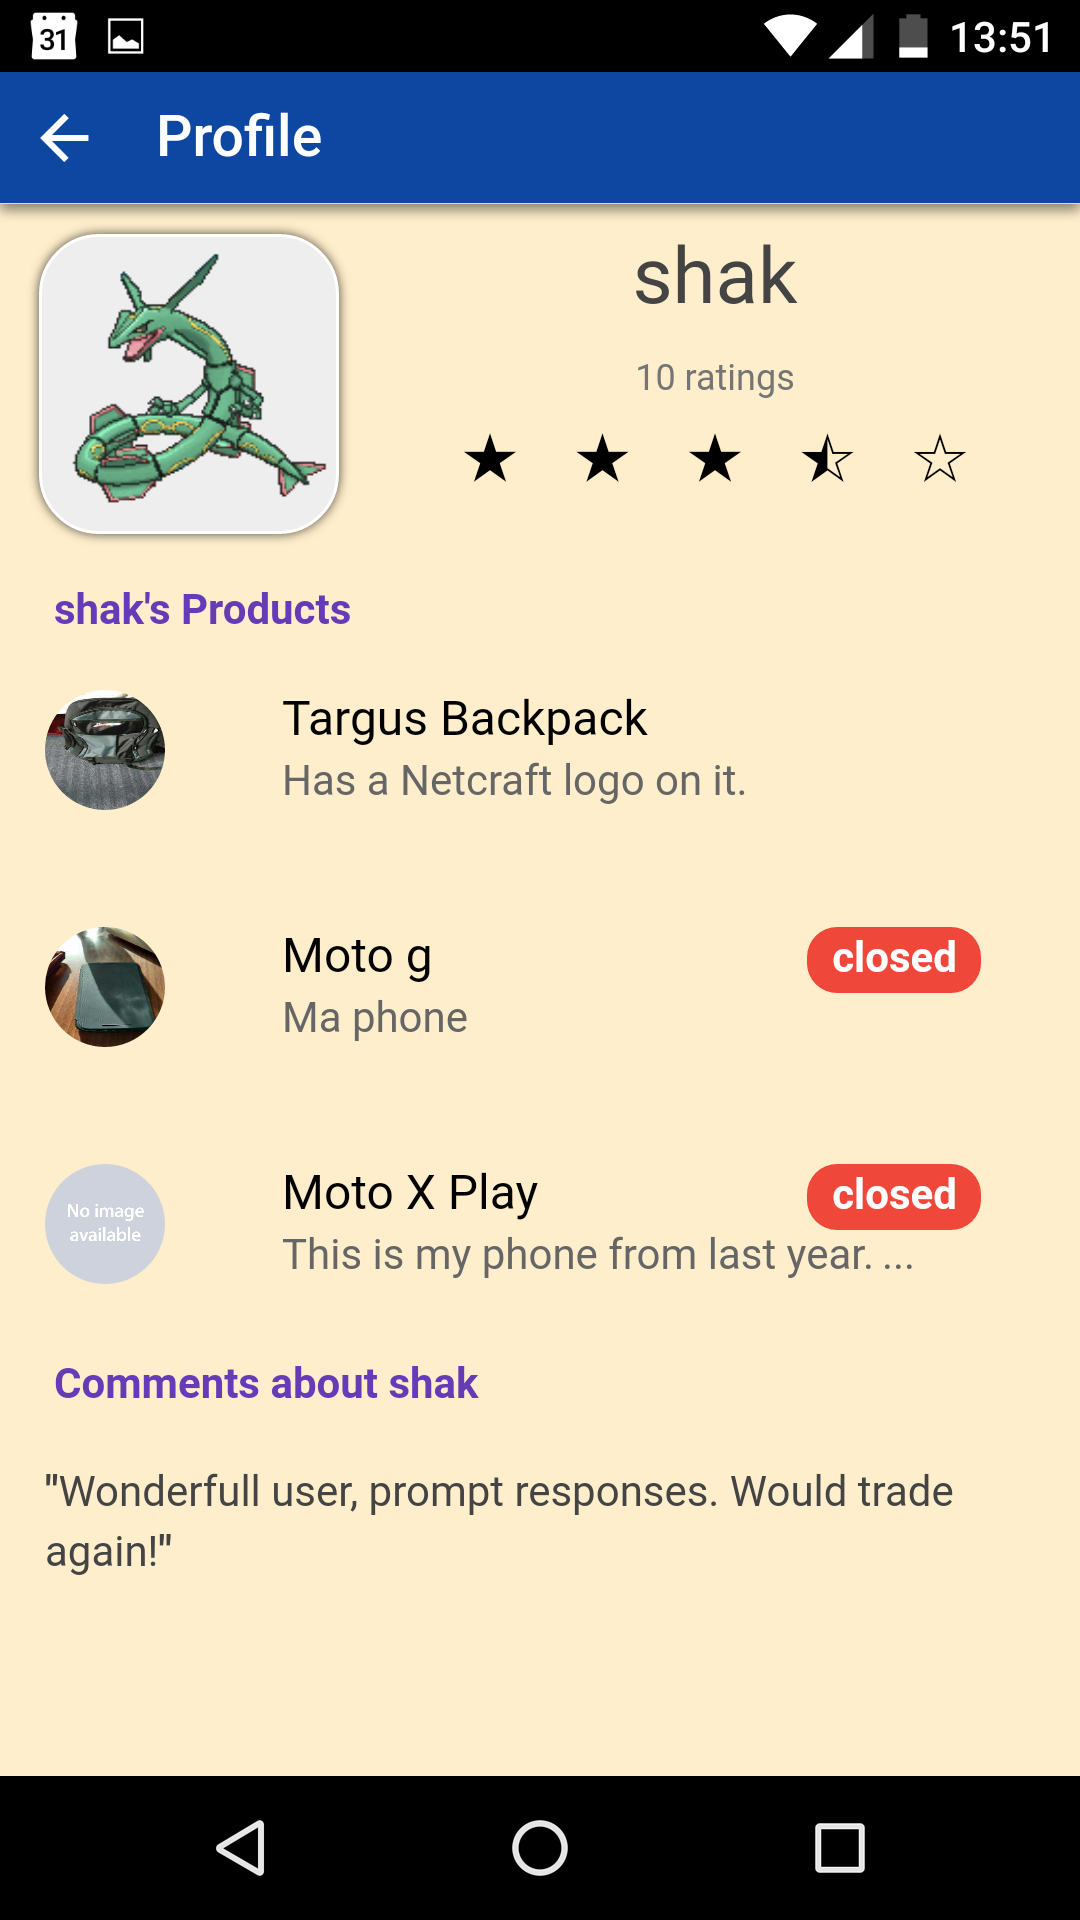
\includegraphics[width=\textwidth]{profile}
        \caption{Profile}
        \label{fig:profile}
    \end{subfigure}
    ~
    \begin{subfigure}[b]{0.3\textwidth}
        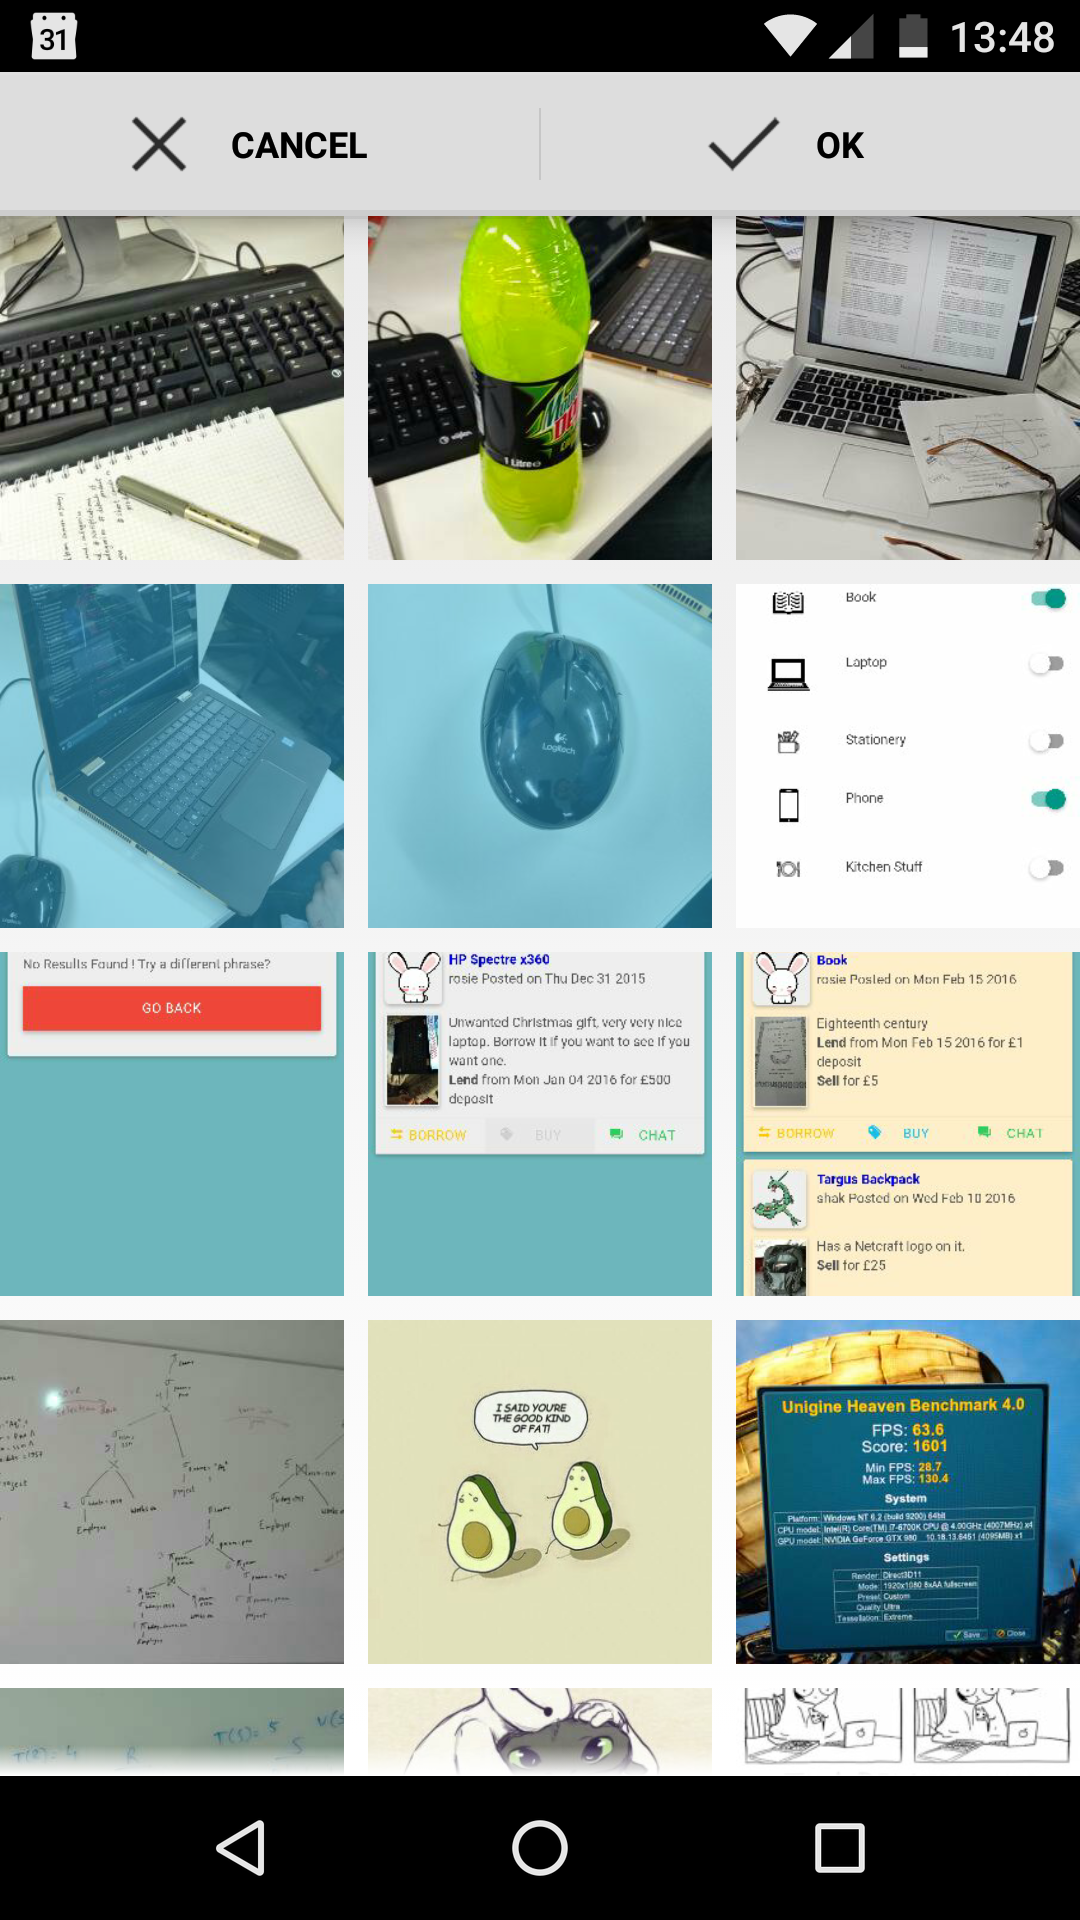
\includegraphics[width=\textwidth]{gallery-select}
        \caption{Gallery Select}
        \label{fig:gallery-select}
    \end{subfigure}
    ~
    \begin{subfigure}[b]{0.3\textwidth}
        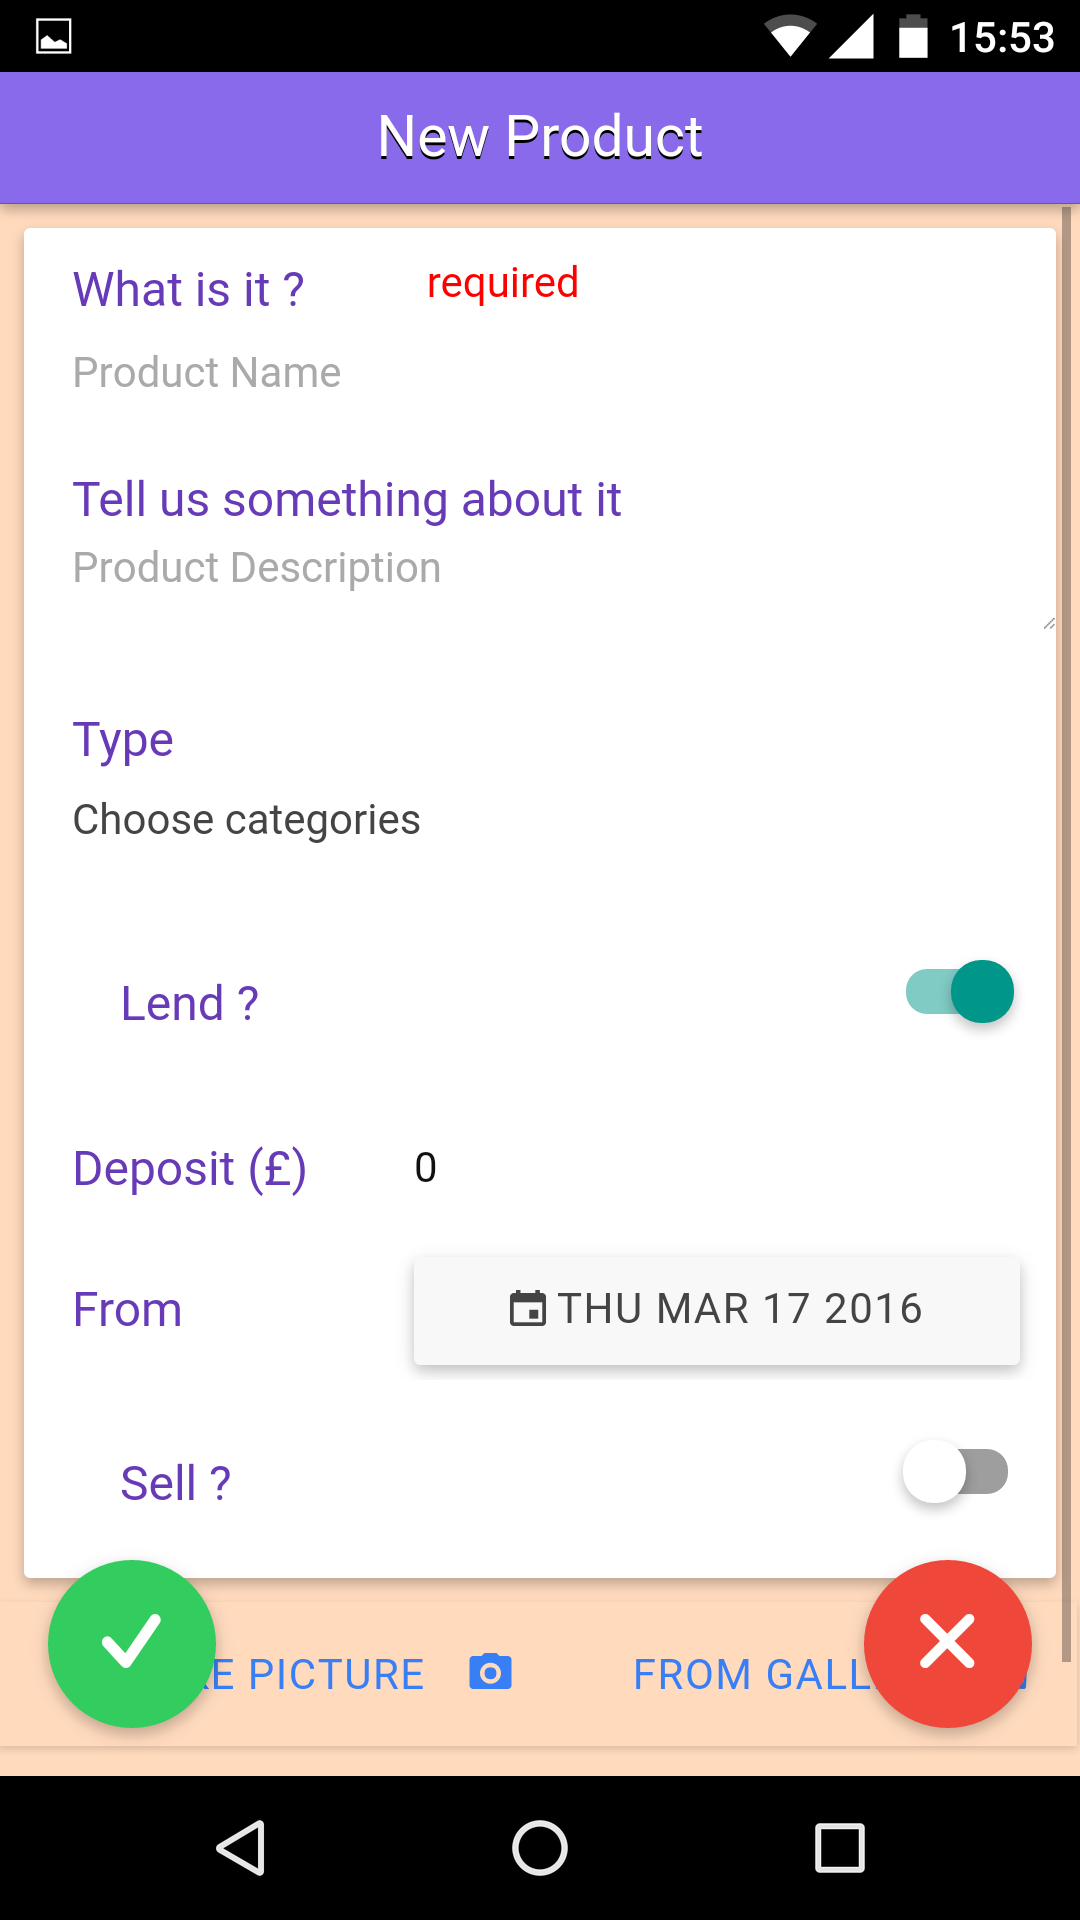
\includegraphics[width=\textwidth]{add}
        \caption{Add Product}
        \label{fig:add}
    \end{subfigure}
    ~
    \begin{subfigure}[b]{0.3\textwidth}
        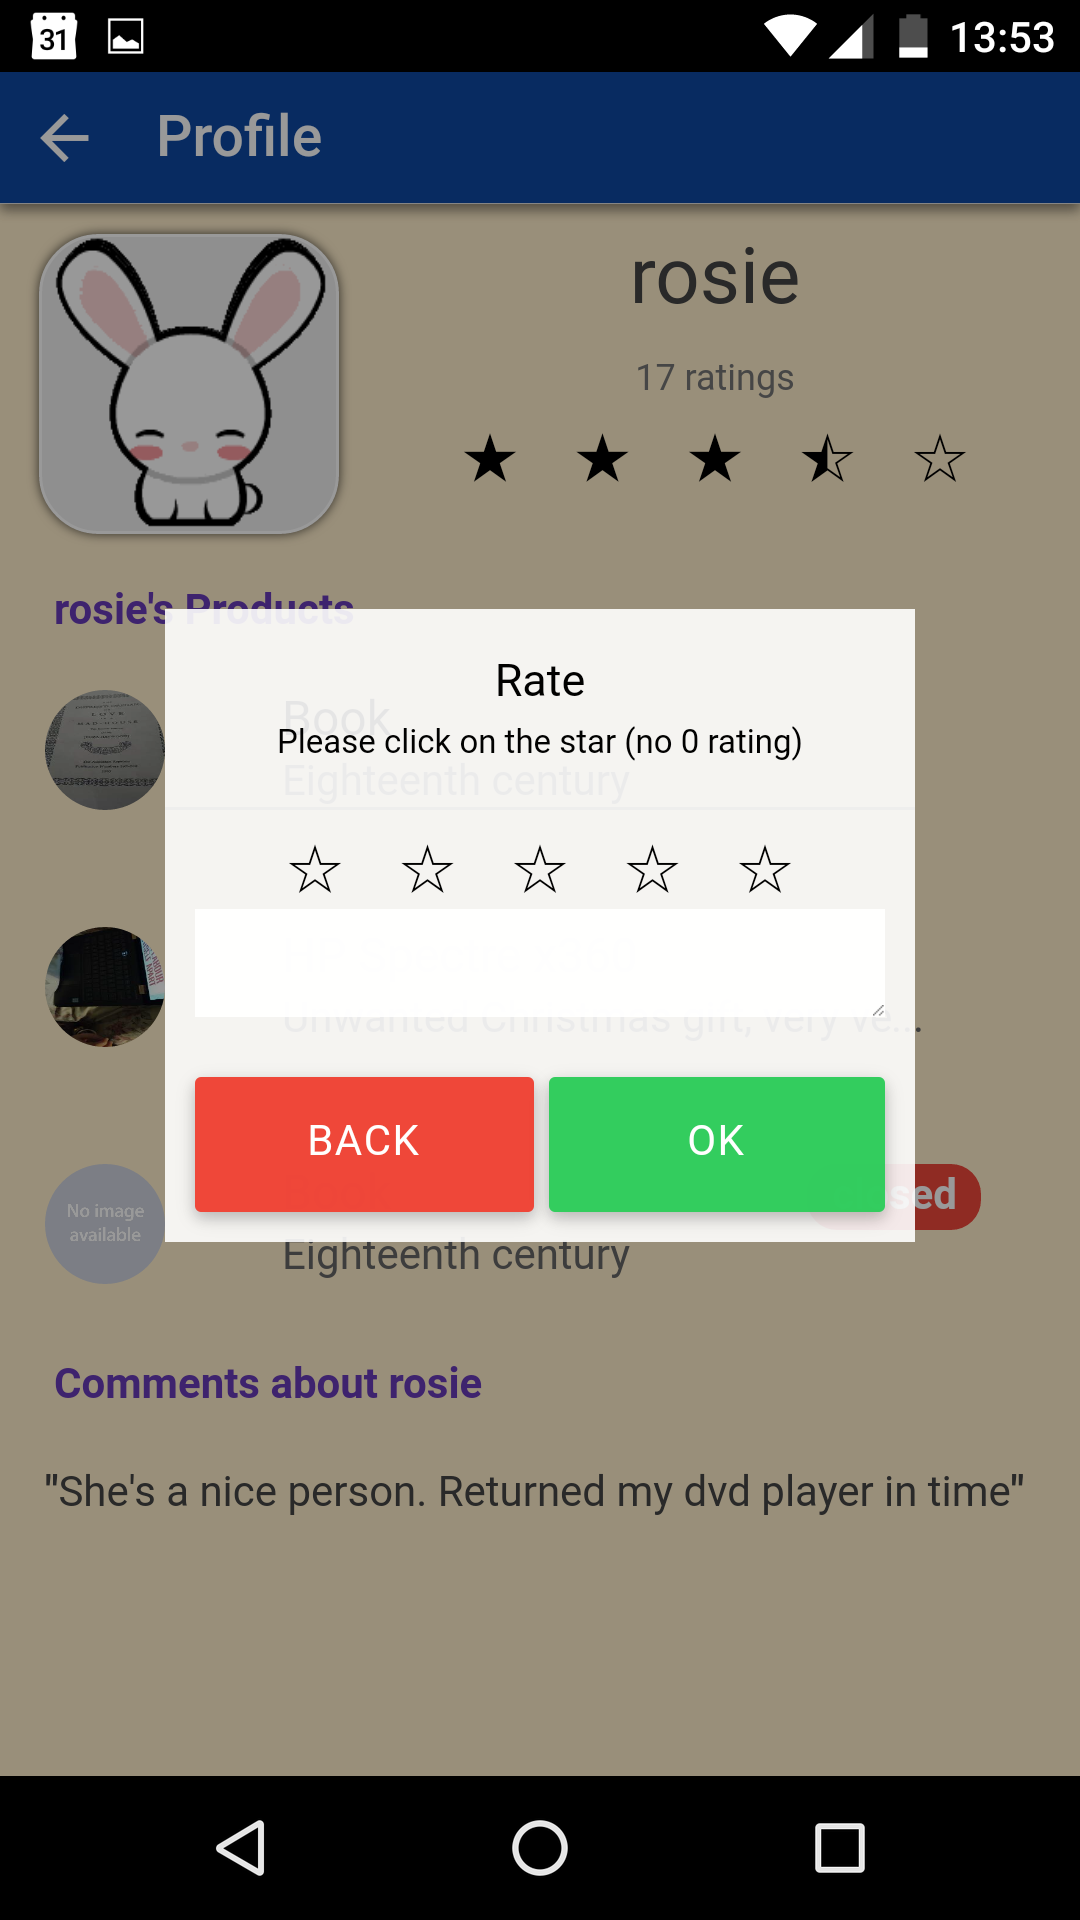
\includegraphics[width=\textwidth]{rate}
        \caption{Rate}
        \label{fig:rate}
    \end{subfigure}
    ~
    \begin{subfigure}[b]{0.3\textwidth}
        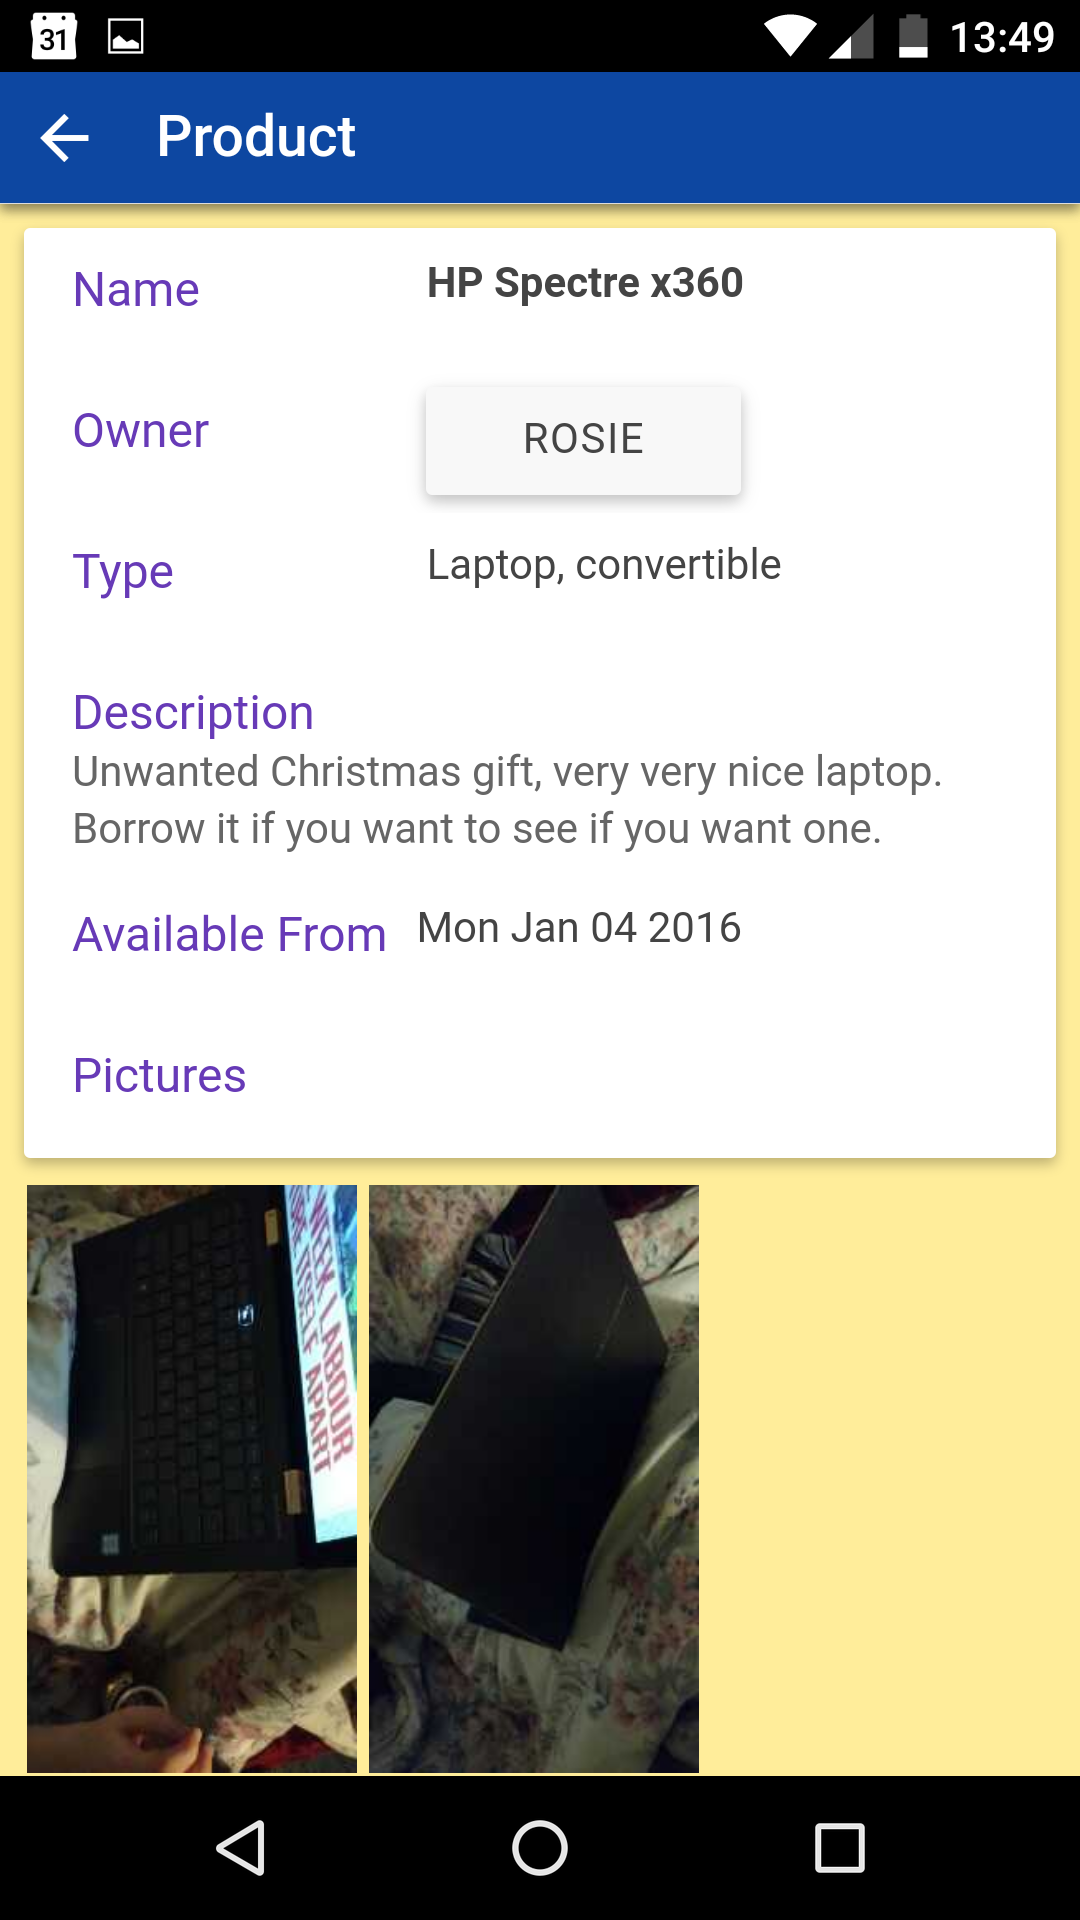
\includegraphics[width=\textwidth]{product}
        \caption{Product Detail}
        \label{fig:product}
    \end{subfigure}
    ~
    \begin{subfigure}[b]{0.3\textwidth}
        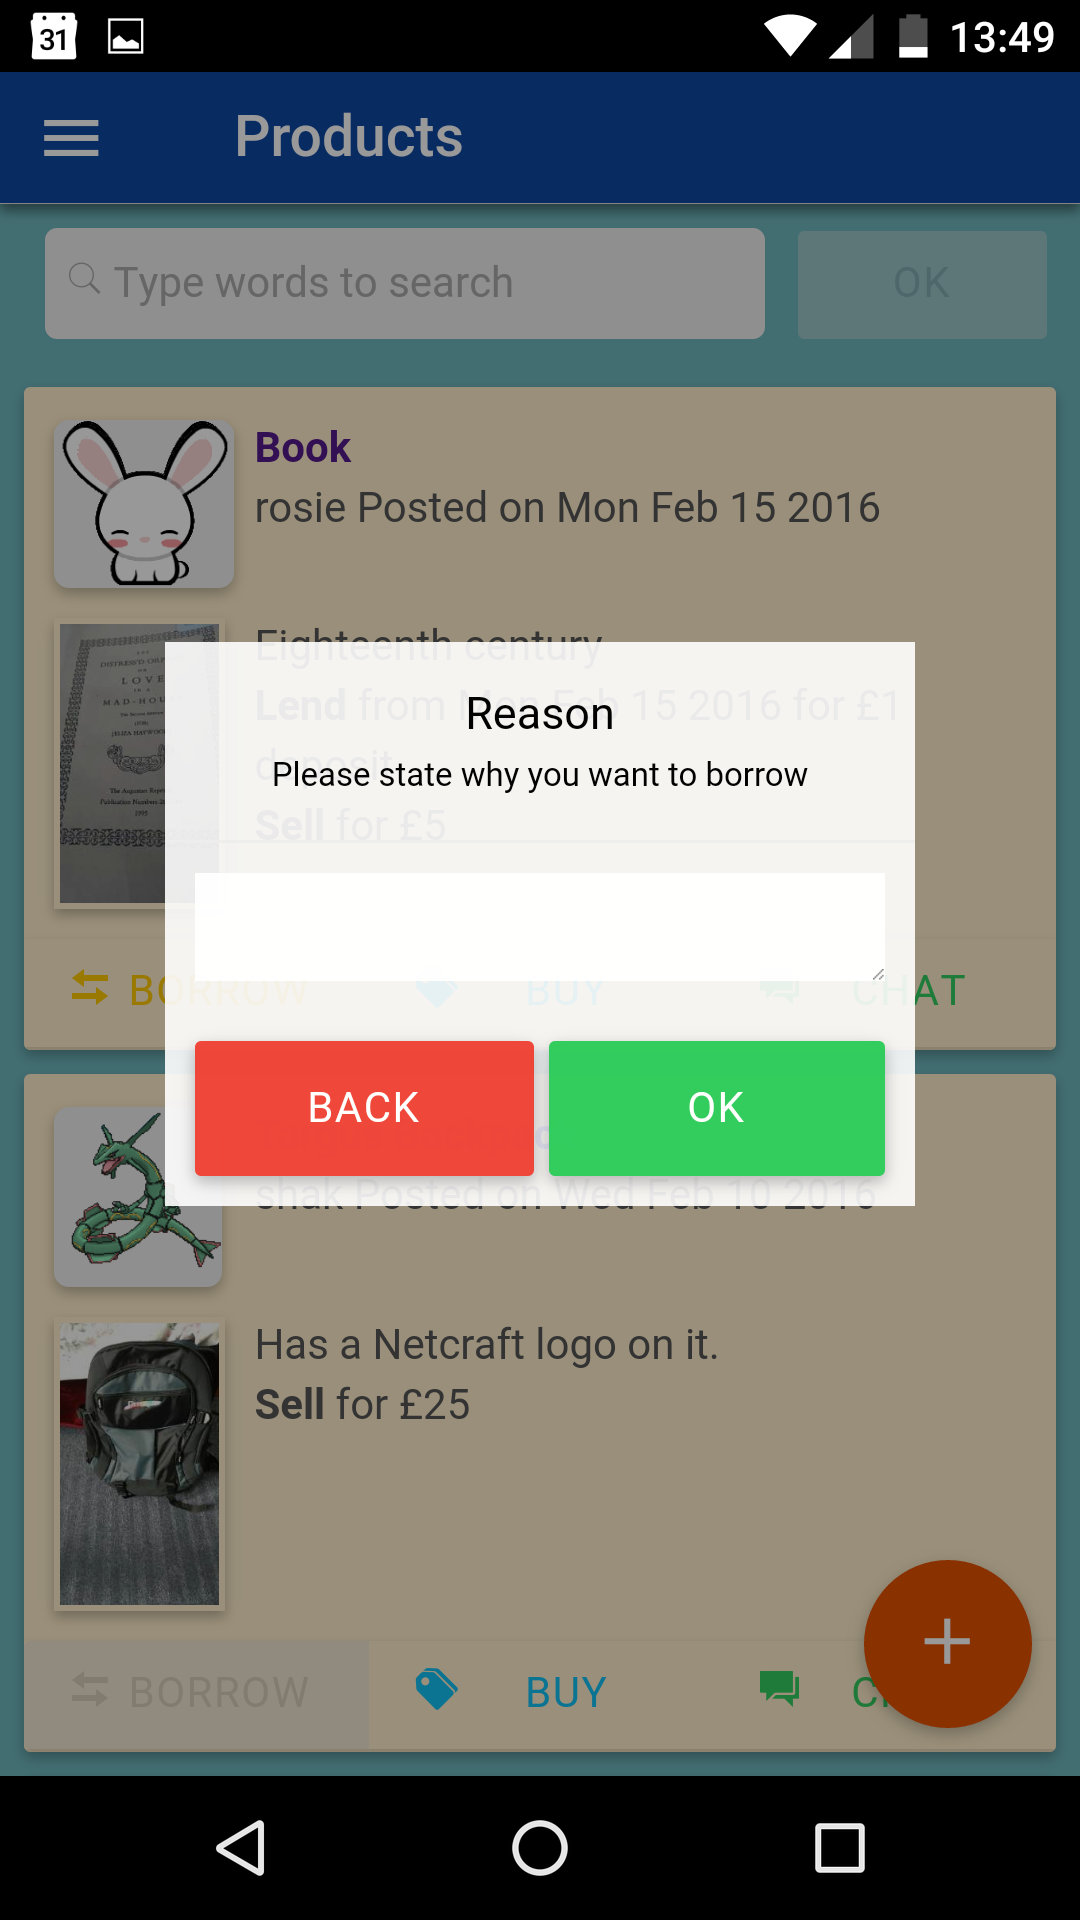
\includegraphics[width=\textwidth]{lend}
        \caption{Borrow}
        \label{fig:lend}
    \end{subfigure}
    ~
    \begin{subfigure}[b]{0.3\textwidth}
        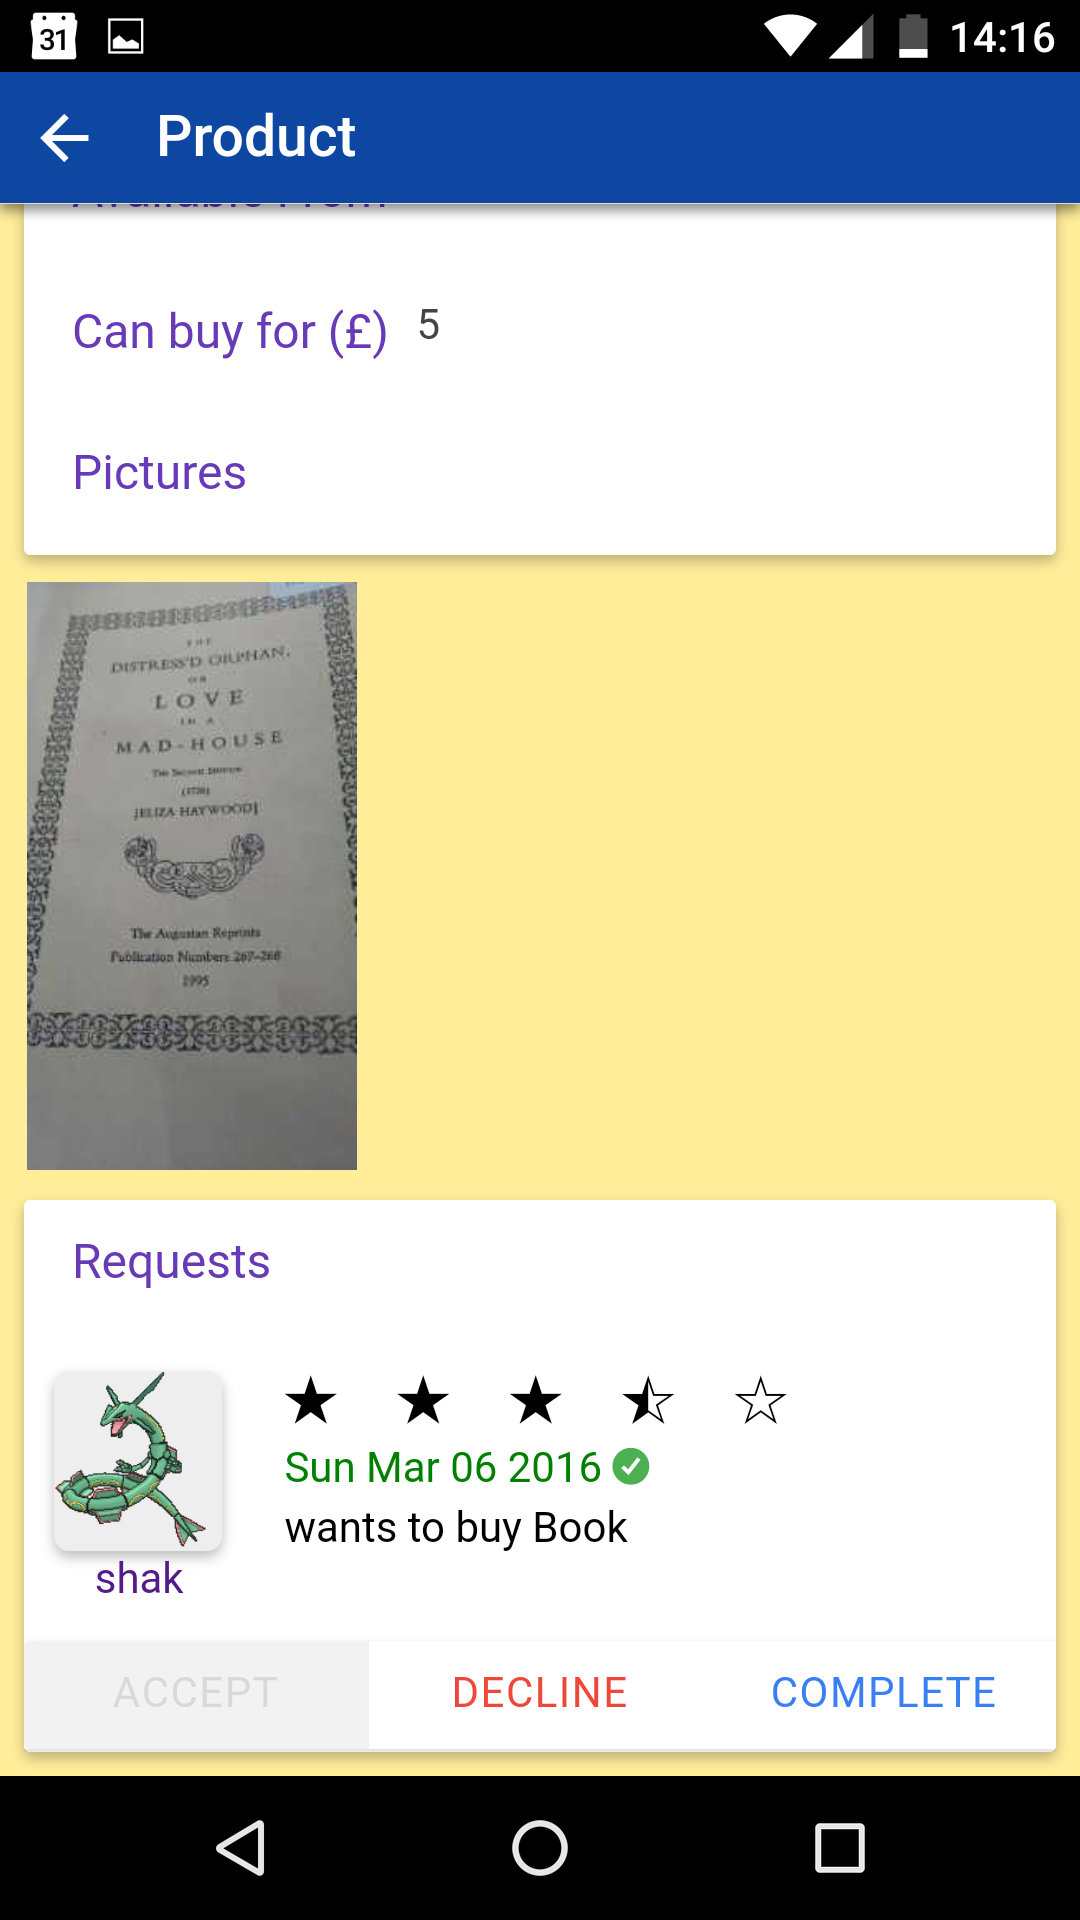
\includegraphics[width=\textwidth]{product-offer}
        \caption{Requests}
        \label{fig:requests}
    \end{subfigure}
    \caption{Screenshots}\label{fig:scr4}
\end{figure}